\chapter{Análise Bibliográfica sobre Simulação e Ensino-Aprendizagem em Sala de Aula, por Jorge Fernandes 2\label{chap:bibliometria:jhcf2}}

\section{Planejamento do estudo\label{STL@jhcf:questoes}}

No caso do meu trabalho, as perguntas que o nortearam foram:
\begin{itemize}
    \item Quais os usos que tem sido feitos de simulação de eventos que ocorrem em sala de aula? 
    \item Que variáveis independentes e dependentes tem sido usadas para o estudo do ensino-aprendizagem? 
    \item Que variáveis independentes e dependentes tem sido usadas para a simulação do ensino-aprendizagem? 
    \item Qual a estrutura social da comunidade que pesquisa sobre o tema?
\end{itemize}

\subsection{O que já existe de pesquisa bibliométrica sobre esse tema?}

Citar ...

\subsection{Uso do Bibliometrix e Biblioshiny}

Foram usadas a ferramenta e o \textit{workflow} proposto pelos autores do pacote Bibliometrix \cite{aria_bibliometrix_2017}.

\subsection{Limitações} O exercício relatado foi feito em uma semana, envolvendo entre x horas de trabalho.

....

\subsection{Registros recuperados}

Doravante o dataset recuperado será chamado de STL@jhcf, que representa o acrônimo Simulation Teach and Learn feito por JHCF.

As informações gerais sobre o dataset STL@jhcf estão sumarizadas na tabela \ref{tab:STL@jhcf:Main}.

\begin{table}[htp]
    \centering
\csvautotabular[separator=comma
%,filter not strcmp={\csvcolii}{}
]{exploratory-data-analysis/jhcf/PesqBibliogr/SimulacaoSalaDeAula/STL@jhcf/Main_Information.csv}
    \caption{Principais dados descritivos do \dataset\ STL@jhcf.}
    \label{tab:STL@jhcf:Main}
\end{table}

A taxa de crescimento anual do dataset foi de 12,45 \%, e o gráfico da figura \ref{STL@jhcf-Crescimento} ilustra o crescimento da publicação entre 1991 e 2022.

\begin{figure}
    \centering
    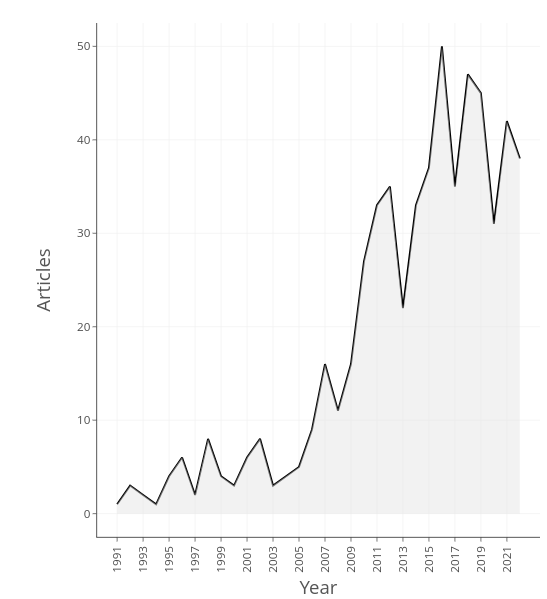
\includegraphics[width=\textwidth]{exploratory-data-analysis/jhcf/PesqBibliogr/SimulacaoSalaDeAula/STL@jhcf/figs/STL@jhcf-Annual-Scientific-Production.png}
    \caption{Evolução de publicações no dataset STL@jhfc.}
    \label{STL@jhcf-Crescimento}
\end{figure}